
The reference implementation %
comprises a \MATLAB{} function \ttt{netcon()}, contained in the file \ttt{netcon.m}, which may be invoked from the \MATLAB{} command line. The performance of this reference implementation may be optionally improved by compiling the C++ component provided in \ttt{netcon\_nondisj\_cpp.cpp}. Assuming that an appropriate compiler has been installed and configured using the \MATLAB{} command \ttt{mex~-setup}, the C++ component may be compiled by typing
\begin{enumerate}
\item[] \ttt{mex netcon\_nondisj\_cpp.cpp}
\end{enumerate}
at the \MATLAB{} command prompt.

Contraction sequences output by \ttt{netcon()} are fully compatible with the tensor network contraction packages \ttt{ncon()} and \ttt{multienv()} of Refs.~\onlinecite{pfeifer2014} and~\onlinecite{evenbly2014} respectively.


\varsubsection{Invocation}

Invocation of the algorithm is via the \MATLAB{} command
\begin{align*}
\ttt{[sequence cost] = netcon(legLinks,verbosity,}\\\ttt{costType,muCap,allowOPs,legCosts);}
\end{align*}
and takes between one and six input parameters, as follows:

\ttt{legLinks}: This parameter describes the tensor network for which an optimal contraction sequence is sought. To construct \ttt{legLinks}, first draw the tensor network using the customary graphical notation (summarised in \S{}1.2 of Ref.~\onlinecite{pfeifer2011a}), with each tensor being represented by a shape, each summed index by a line connecting the two tensors on which it appears, and each unsummed index by a line with one free end and the other end attached to the tensor on which it appears\arXtext{ [for example,~\fref{fig:31MERA} is a graphical representation of Eq.~\eref{eq:31MERA}]}.
Next, label each summed index with a unique positive integer, and each unsummed index with a unique negative integer, descending consecutively from $-1$ (e.g.~\fref{fig:labelled31MERA}). 
\begin{figure}
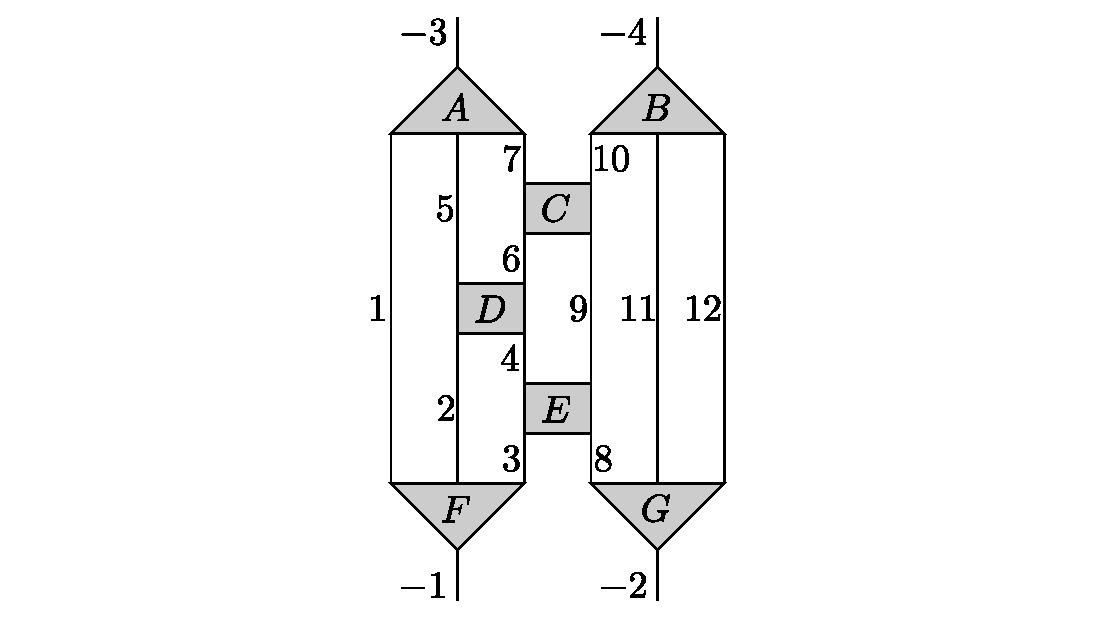
\includegraphics[width=246.0pt]{labelled31MERA}
\caption{\label{fig:labelled31MERA}A tensor network is described to \ttt{netcon()} using labelled indices. In this diagram,\arXtext{ which shows the same tensor network as \pfref{fig:31MERA},} summed indices have been labelled with unique positive integers, and open indices have been labelled with unique negative integers descending consecutively from $-1$. The tensors have also been labelled with letters to allow easy reference from the text.}
\end{figure}%
For each tensor~$T$, now construct a $1\times n_T$ matrix where $n_T$ is the number of indices attached to tensor~$T$, with entries corresponding to the labels associated with those indices. Ordering of the indices is unimportant. If there are $m$ tensors, then there are $m$ such matrices, which may be denoted $M_i,~i\in\{1\ldots m\}$.
Finally, \ttt{legLinks} comprises a $1\times m$ cell array, with the $m$ entries of this array corresponding to the matrices $M_i$, with ordering once again being unimportant. For example, the labelling given in \fref{fig:labelled31MERA} may be associated with the input parameter
\begin{align*}
\ttt{legLinks~=~\{}&\ttt{[-1 1 2 3],[2 4 5 6],[1 5 7 -3],}\\
&\ttt{[3 8 4 9],[6 9 7 10],[-2 8 11 12],}\\
&\ttt{[10 11 12 -4]\}}.
\end{align*}

\ttt{verbosity}: Determines the level of output generated by \ttt{netcon()}. For $\ttt{verbosity}=0$, an optimal index contraction sequence is returned in \ttt{sequence} and the associated cost is returned in \ttt{cost} but operation is otherwise silent. For $\ttt{verbosity}=1$, a message is generated every time the upper bound on tensor contraction costs is increased as described in \srefp{sec:costcap}, and on completion an optimal sequence and the associated cost are displayed on screen. For $\ttt{verbosity}=2$, behaviour is as for $\ttt{verbosity}=1$ but candidate contraction sequences and associated costs are announced when these sequences constitute the lowest-cost contraction sequence found so far. The final sequence and cost announced then correspond to the optimal solution reported at $\ttt{verbosity}=1$ and returned in the output variables \ttt{sequence} and \ttt{cost}. Setting $\ttt{verbosity}=3$ displays additional information about the pairwise contractions being performed. %

\ttt{costType}: To determine an optimal contraction sequence associated with a given tensor network, it is necessary to specify the dimension of each index in the network. Index dimensions may either be specified as integers, or in the form $a\chi^b$, where $\chi$ is an unspecified parameter which is presumed to be large. The former is indicated by $\ttt{costType}=1$, and the latter by $\ttt{costType}=2$. Default value: 2. Note that
when using $\ttt{costType}=2$, indices of some fixed dimension $d$ (such as the physical indices of an MPS or PEPS) may be represented by setting $a=d$ and $b=0$.

\ttt{muCap}: When searching for an optimal contraction sequence, \ttt{netcon()} initially restricts itself to sequences having a cost of at most $\xicap$ (for $\ttt{costType}=1$) or $\OO{\chi^\xicap}$ (for $\ttt{costType}=2$), where \ttt{muCap} represents $\xicap$. The value of \ttt{muCap} will automatically increase if no contraction sequence exists which satisfies this constraint. Setting \ttt{muCap} too high can incur extremely large overheads, whereas the process of automatic increase is relatively low-cost due to the caching of data in $S_i$ described in Secs.~\ref{sec:breadthalg} and \refp{sec:costcap}. It is therefore recommended that \ttt{muCap} be left at its default value of 1 unless the cost to contract the network is already known.

\ttt{allowOPs}: Determines whether \ttt{netcon()} should examine contraction sequences involving outer products (e.g.~$A^\alpha_\beta B^\gamma_\delta=C^{\alpha\gamma}_{\beta\delta}$). For tensor networks where there exists an optimal contraction sequence which does not involve an outer product, setting \ttt{allowOPs} to \ttt{false} may result in faster performance. However, if an outer product is required to obtain an optimal contraction sequence, this will also result in a suboptimal sequence being returned. Default value: \ttt{true}.



\ttt{legCosts}: The format of this input parameter is dependent upon the value of \ttt{costType}.
\begin{enumerate}
\item For $\ttt{costType}=1$, \ttt{legCosts} is an $\ell\times 2$ matrix whose first column consists of index labels and whose second column gives the dimensions associated with those labels. If \ttt{legCosts} is not specified, it is assumed that each index has dimension 2. 
\item For $\ttt{costType}=2$, \ttt{legCosts} comprises an $\ell\times 3$ matrix where $\ell$ is the total number of unique index labels. Each row then comprises three entries, $[x~a~b]$, where $x$ is a index label (and hence a positive or negative integer), and $a$ and $b$ specify the dimension of index $x$ in terms of the cost parameter $\chi$, such that $\mrm{dim}(x)=a\chi^b$. If \ttt{legCosts} is not specified, it is assumed that each index (whether summed or unsummed) has dimension $\chi$. Note that $b$ may take the value zero, permitting a fixed cost to be specified for some indices. 
\end{enumerate}
Regardless of the value of \ttt{costType}, if \ttt{legCosts} is specified, each index label must appear in the first column precisely once. Note that tensors of total dimension~1 are not supported.




On completion, \ttt{netcon()} returns an optimal contraction sequence and associated cost. These are specified as follows:

\ttt{sequence}: Sequence over which the indices of the tensor network should be summed in order to contract the network for minimum cost. For the interpretation of this sequence, see \condaref{sec:sequencenotation}.

\ttt{cost}: Specifies the total number of multiplication operations associated with optimal contraction of the tensor network, for example according to the sequence returned in \ttt{sequence}. For $\ttt{costType}=2$ this value is a number. For $\ttt{costType}=1$ the cost takes the form of a polynomial in $\chi$,
\begin{equation}
\sum_{i=0}^{\chi_\mrm{max}}a_i\chi^i,
\end{equation}
and this is returned as a $1\times \chi_\mrm{max}$ array whose entries \ttt{cost(i)} correspond to the coefficients $a_{i-1}$. %

Note that when a tensor network involves one or more traces, these may always be evaluated before network contraction begins. Evaluating a trace involves only addition operations, not multiplication, and thus these operations are relatively cheap and are ignored when computing the value of \ttt{cost} (though the presence of costs associated with tracing over indices will be noted in the text output if $\ttt{verbosity}>0$). %

\varsubsection{Index sequence notation\label{sec:sequencenotation}}

In the main body of this paper we have employed a heirarchical tensor-based notation to describe sequences of tensor contractions, with $((AB)C)$ indicating the contraction of tensor $A$ with tensor $B$ over all common indices (if any), followed by the contraction of the resulting object with tensor $C$. This notation is clear, unambiguous, and easily human-readable. In software implementations of tensor network algorithms, however, a linear notation is more widely used.

In this notation the indices of the tensor network are labelled as in \fref{fig:labelled31MERA}, and contractions are described by specifying the order in which the index sums are to be performed. For example, in the sequence
\begin{equation}
\ttt{[11 12 9 4 6 5 7 1 2 3 8 10]}
\end{equation}
the first sums are over indices 11 and 12, corresponding to contraction of tensor $B$ of \fref{fig:labelled31MERA} with tensor $G$. The next is over index 9, corresponding to contraction of tensor $C$ with tensor $E$. Proceeding in this fashion, the sequence is seen to describe the tensor contraction
\begin{equation}
((BG)((((CE)D)A)F)).
\end{equation}

Using an index-based notation it is also possible to describe sequences having no direct counterpart in the pairwise tensor contraction notation, for example
\begin{equation}
\ttt{[11 9 4 6 5 7 1 2 3 8 10 12]}.\label{eq:deferredtrace}
\end{equation}
In this contraction sequence, tensors $B$ and $G$ are combined by contracting over index~11 but index~12 remains unsummed until the end of the contraction sequence. In conventional tensor notation, writing $T$ for $(BG)$, one may write
\begin{equation}
T^{aef}_{bdg}=B^a_{bcd}G^{ecf}_g\label{eq:suboptimal}
\end{equation}
but the subsequent contraction over index~12 implies that we need only compute the diagonal elements
\begin{equation}
T^{aed}_{bdg}=B^a_{bcd}G^{ecd}_g,\qquad\textrm{no sum over $d$,}\label{eq:sparsetensor}
\end{equation}
similar to the calculation of $\left(C^*\right)^l_{ijkl}$ in \Erefp{eq:lunsummed}. However, as noted in \srefp{sec:flops} and in \rcite{lam1997}, it is never suboptimal to immediately sum such a repeated index. The behaviour of tensor contraction software for index sequences such as that in \Eref{eq:deferredtrace} may vary, with possibilities including producing a warning and performing the suboptimal contraction of \Eref{eq:suboptimal}, pre-emptive contraction of index~12 at the same time as index~11 regardless of the supplied sequence, or construction of a sparsely-populated tensor diagonal in index~12 as per \Eref{eq:sparsetensor}. To avoid this ambiguity, \ttt{netcon()} always returns sequences in which all index contractions between a given pair of tensors are performed at the same time. (An exception is made for indices of dimension one---the special handling of these indices is described in \condaref{sec:subnets}).

We also find it necessary to introduce an extension to the usual index sequence notation in order to describe tensor contraction sequences involving outer products. Although this notation is not universal---it cannot describe an entirely arbitrary contraction sequences involving outer products---it nevertheless suffices to describe all outer products consistent with the restrictions of \srefp{sec:restrictops}, and thus there always exists an optimal contraction sequence which can be expressed in this form.

In this extension, we use the label~0 to denote an outer product between two tensors, with a string of $n$ zeros denoting $n$ outer product operations between a total of $n+1$ tensors. These tensors are identified as follows:
\begin{itemize}
\item If there are $n$ zeros and only $n+1$ tensors remaining to contract, the outer product is between all remaining tensors.
\item Otherwise, read indices from the sequence following the zeros, and note the tensors they belong to, until $n+2$ tensors have been identified. By \scref{item:(AB)noopC} in \srefp{sec:tensorsinOP}, these $n+2$ tensors will comprise $n+1$ tensors participating in the outer product, and one tensor which shares indices with all of the other $n+1$ tensors. Perform the outer product on the $n+1$ tensors thus identified.
\end{itemize}
Outer products on multiple tensors should be performed pairwise, always acting on the two tensors of smallest total dimension.

An example tensor network requiring an outer product for optimal contraction is given in \fref{fig:disjointsequence}.
\begin{figure}
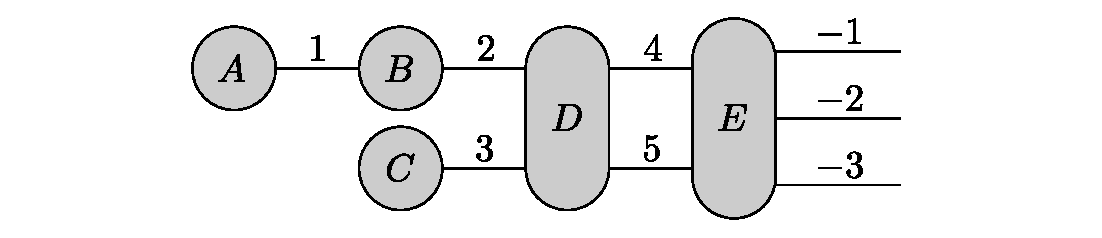
\includegraphics[width=246.0pt]{disjointsequence}
\caption{An example tensor network for which the optimal contraction sequence involves performing an outer product. All indices are of dimension $\chi$, with $\chi>1$.\label{fig:disjointsequence}}
\end{figure}%
The optimal contraction sequence for this network, in index notation, is
\begin{equation*}
\ttt{[1 0 2 3 4 5]}
\end{equation*}
which corresponds to a pairwise tensor contraction sequence of
$((((AB)C)D)E)$.

A detailed algorithm for parsing index-based contraction sequences, including sequences which contain zeros to denote outer products, is provided for reference in \condaref{sec:readingsequence}. The syntax described, including the use of zeros to denote outer products, is fully supported by the tensor network contraction packages \ttt{ncon()} and \ttt{multienv()} of Refs.~\onlinecite{pfeifer2014} and~\onlinecite{evenbly2014} respectively.

\varsubsection{Disjoint subnetworks\label{sec:subnets}}

A tensor network is described as disjoint if it may be written as two or more factors sharing no common indices, e.g.~\Erefp{eq:disjoint}. Where a network is made up of multiple disjoint components, it is almost always preferable to address each component individually (with the only caveat relating to components which reduce to a scalar, as discussed in footnote~\refp{fn:scalar}). While, strictly speaking, the handling of such networks lies outside the scope of a reference implementation of the algorithm of \aref{sec:pseudocode}, support for disjoint networks has nevertheless been included in the interest of providing an implementation of maximal usefulness to the tensor network community. Each subnetwork is processed individually, and the resulting contraction sequences are concatenated together using outer products, represented by a string of zeros at the end of the contraction sequence.

As the computational cost of finding an optimal contraction sequence scales non-polynomially in $N$, the number of tensors, there is substantial benefit to be gained by identifying disjoint subnetworks and treating them independently. In light of this, it is noted that summing over an index of dimension one is formally equivalent to performing an outer product. For example, a column vector may be denoted either $A^a$ or $A^a_b$ where the only admissible value for index $b$ is 1, and the calculation
\begin{equation}
C^a_c = A^a_b B^b_c
\end{equation}
is entirely equivalent to
\begin{equation}
C^a_c = A^a B_c.
\end{equation}
Provided outer products between disconnected tensors are considered as part of a search algorithm, there is no disadvantage to ignoring or deleting all summed indices of dimension one in a tensor network. The reference implementation of \ttt{netcon()} ignores the existence of these indices both when identifying disjoint subnetworks and when determining optimal contraction sequences, and defers the zero-cost action of ``tracing over all indices of dimension one'' until the very end of the index contraction sequence. Because these indices are of dimension one there is never any cost penalty associated with doing so, even given the most pessimistic interpretation of contraction sequence notation as illustrated in \Eref{eq:suboptimal}.

\varsubsection{Sample invocation and output}

As a simple example, consider the tensor network given in \fref{fig:labelled31MERA}. Allowing \ttt{costType} and \ttt{legCosts} to take their default values, corresponding to each index having dimension $\chi$, \ttt{netcon()} may be invoked with verbosity level 1 by the command
\begin{align*}
\ttt{[sequence cost]=netcon(\{}&\ttt{[-1 1 2 3],[2 4 5 6],}\\
&\ttt{[1 5 7 -3],[3 8 4 9],}\\
&\ttt{[6 9 7 10],[-2 8 11 12],}\\
&\ttt{[10 11 12 -4]\},1);}
\end{align*}
with the pure-\MATLAB{} version returning the output
\begin{verbatim}
Looking for solutions of cost O(X^1)
Looking for solutions of cost O(X^6)
Looking for solutions of cost O(X^7)
Looking for solutions of cost O(X^8)
 
Best sequence:   11 12 9 4 6 5 7 1 2 3 8 10
Cost:            2X^8 + 2X^7 + 2X^6 + 0X^5
                 + 0X^4 + 0X^3 + 0X^2 + 0X^1
                 + 0X^0
\end{verbatim}
indicating that the cost of contracting this network scales as $\mrm{O}(\chi^8)$, and that for any given value of $\chi$ the actual cost of performing this contraction will be $2\chi^8+2\chi^7+2\chi^6$. The sequence and cost are also returned in the variables \ttt{sequence} and \ttt{cost}:
\begin{equation*}
\begin{tabular}{l}
\ttt{sequence = [11 12 9 4 6 5 7 1 2 3 8 10]}\\
\ttt{cost~~~~~= [0 0 0 0 0 0 2 2 2]}.
\end{tabular}
\end{equation*}
(Note that the pure-\MATLAB{} and \MATLAB{}-and-C++ versions use different methods of internally tabulating the results of intermediate contractions and so will frequently return different sequences to one another, but with the same contraction cost. This is because each version returns the first sequence of optimal cost which it encounters, and this may vary depending upon the order in which all relevant contractions are explored.)

\varsubsection{Using \ttt{netcon()} with \ttt{multienv()}}

The reference implementation of the ideas presented in this paper, \ttt{netcon()}, produces output compatible with the \ttt{multienv()} package described in \rcite{evenbly2014}. However, the networks supplied to \ttt{multienv()} are always \emph{closed} networks (i.e.~with no uncontracted indices), and we can take advantage of this. The \ttt{multienv()} package does not require an optimal contraction sequence for the supplied network, only a contraction sequence in the optimal \emph{family}, as defined in \rcite{evenbly2014}. This may be obtained at cheaper computational cost by deleting one tensor from the network, using \ttt{netcon()} to determine an optimal sequence for the open network, and finally reintroducing the deleted tensor, with contraction over the indices on this tensor being the final step in the contraction of the closed tensor network. A sequence obtained in this manner, while not necessarily optimal for contraction of the entire closed network, is nevertheless a member of the optimal family of sequences, and suffices for \ttt{multienv()} to calculate all requested tensor environments at minimal cost.

\section{Interpretation of contraction sequences specified as a list of indices\label{sec:readingsequence}}

The \ttt{netcon()} algorithm described in this paper takes as its input a description of a tensor network where each summed index is associated with a positive integer label and each open index is associated with a negative integer label. As its output the algorithm returns an optimal contraction sequence for the specified tensor network, specified as a list of
positive integer labels possibly interspersed with zeros,
and the cost of performing this contraction (corresponding to the number of multiplication operations required). 
Interpretation of tensor contraction sequences specified in this form is described in the paper above, but is summarised in this Appendix for convenience.

Starting with a list of tensors in the network to be contracted, and beginning with the first index of the sequence, contraction of a tensor network proceeds as follows:
\begin{description}[align=left,font=\normalfont,itemsep=2pt]
\item[1] If the sequence list is empty, stop. Contraction of the tensor network is complete.
\item[2] Read the first entry, $i_1$. 
\item[3] If $i_1=0$:
\begin{description}[align=left,font=\normalfont,itemsep=2pt]
\item[3a] Read a further $x-1$ entries, for a total of $x$ entries, denoted $i_1,\ldots,i_x$, where $x$ is the largest possible value such that all $x$ entries are zero.
\item[3b] Let $n$ be the number of tensors currently in the list of tensors. If $x=n-1$:
\begin{description}[align=left,font=\normalfont,itemsep=2pt]
\item[3b1] Using the outer product algorithm given below, perform an outer product of all $n$ remaining tensors. Denote the result of this outer product $X$. Delete all $n$ tensors from the list. Add tensor~$X$ to the list.
\item[3b2] Delete entries $i_1,\ldots,i_x$ from the sequence.
\item[3b3] Go to step 1.
\end{description}
\item[3c] Otherwise (i.e.~$x\not=n-1$):
\begin{description}[align=left,font=\normalfont,itemsep=2pt]
\item[3c1] Delete entries $i_1,\ldots,i_x$ from the sequence.
\item[3c2] Read the next $y$ entries from the sequence (denoted $j_1,\ldots,j_y$), and list all tensors on which indices $j_1,\ldots,j_y$ appear, where $y$ is the largest possible value such that all entries $j_1,\ldots,j_y$ are nonzero and the number of tensors in the list is precisely $x+2$.
\item[3c3] Let these tensors be referred to as ${A}_1,\ldots,{A}_{x+2}$.
\item[3c4] Let ${B}_1$ and ${B}_2$ denote the tensors on which index $j_1$ appears. Identify the smallest value of $z$ such that index $j_z$ appears on a tensor which is neither ${B}_1$ nor ${B}_2$. Index $j_z$ also appears on either ${B}_1$ or ${B}_2$. Let $X$ denote this tensor (either ${B}_1$ or ${B}_2$). Note that tensor~$X$ will be a member of the list ${A}_1,\ldots,{A}_{x+2}$.
\item[3c5] Using the outer product algorithm given below, perform an outer product of all tensors ${A}_1,\ldots,{A}_{x+2}$ except for tensor~$X$. Let the result of this outer product be denoted $Y$.
\item[3c6] Indices $j_1,\ldots,j_y$ all appear on both $X$ and $Y$. Evaluate the product of tensors~$X$ and $Y$, denoted $(XY)$, summing over all possible configurations of the indices $j_1,\ldots,j_y$.
\item[3c7] Delete tensors~${A}_1,\ldots,{A}_{x+2}$ from the list of tensors. Add tensor $(XY)$ to the list of tensors.
\item[3c8] Delete indices $j_1,\ldots,j_y$ from the sequence.
\item[3c9] Return to step 1.
\end{description}
\end{description}
\item[4] Otherwise (i.e.~$i_1\not=0$), identify which tensors index $i_1$ appears on.
\item[5] If index $i_1$ appears on only one tensor, it represents a trace. Read a further $x-1$ indices, for a total of $x$ indices, denoted $i_1,\ldots,i_x$, where $x$ is the largest possible value such that indices $i_1,\ldots,i_x$ are all traces and all appear on the same tensor. Trace over indices $i_1,\ldots,i_x$, delete these indices from the sequence, and return to step~1. (It is permissible for $x-1$ to be zero.)
\item[6] Otherwise: Index $i_1$ appears on two tensors, $A$ and $B$. Read a further $x-1$ indices, for a total of $x$ indices, denoted $i_1,\ldots,i_x$, where $x$ is the largest possible value such that all indices $i_1,\ldots,i_x$ appear on both tensor~$A$ and tensor~$B$. (It is permissible for $x-1$ to be zero.)
\item[7] Evaluate the product of tensors~$A$ and $B$, denoted $(AB)$, summing over all possible configurations of the indices $i_1,\ldots,i_x$.
\item[8] Delete tensors~$A$ and $B$ from the list of tensors. Add tensor $(AB)$ to the list of tensors.
\item[9] Delete indices $i_1,\ldots,i_x$ from the sequence.
\item[10] Return to step 1.
\end{description}

When called upon to perform an outer product of $m$ tensors, this should be done by applying the following algorithm:
\begin{description}[align=left,font=\normalfont]
\item[1] Define the total dimension of a tensor as the product of the dimensions of its indices.
\item[2] List the $m$ participating tensors.
\item[3] Identify the two tensors having the smallest total dimensions.
\item[4] Remove those two tensors from the list.
\item[5] Add their outer product to the list.
\item[6] Repeat steps 3-5 until only one tensor remains.
\end{description}
